\section{Derivatives and Integrals of Vector-Valued Functions} \label{S:9.7.Vector_Valued_Functions_Derivatives}
 
\vspace*{-14 pt} \framebox{\hspace*{3 pt}
\parbox{6.25 in}{\begin{goals}
\item What do we mean by the derivative of a vector-valued function
and how do we calculate it?
\item What does the derivative of a vector-valued function measure?
\item What do we mean by the integral of a vector-valued function and
how do we compute it?
\item How do we describe the motion of a projectile if the only force
acting on the object is acceleration due to gravity?
\end{goals}} \hspace*{3 pt}}

\subsection*{Introduction}

A vector-valued function $\vr$ determines a curve in space as the
collection of terminal points of the vectors $\vr(t)$. If the curve is
smooth, it is natural to ask whether $\vr(t)$ has a derivative.  In
the same way, our experiences with integrals in single-variable
calculus prompt us to wonder what the integral of a vector-valued
function might be and what it might tell us.  We
explore both of these questions in detail in this section.

For now, let's recall some important ideas from calculus I.  Given a
function $s$ that measures the position of an object moving along
an axis, its derivative, $s'$, is defined by
$$s'(t) = \lim_{h \to 0} \frac{s(t+h) - s(t)}{h},$$
and measures the instantaneous rate of change of $s$ with respect to
time.  In particular, for a fixed value $t = a$, $s'(a)$ measures the
velocity of the moving object, as well as the slope of the tangent
line to the curve $y = s(t)$ at the point $(a,s(a))$.

As we work with vector-valued functions, we will strive to update
these ideas and perspectives into the context of curves in space and
outputs that are vectors.

\begin{pa} \label{PA:9.7} Let $\vr(t) = \cos(t) \vi + \sin(2t) \vj$ describe the path traveled by an object at time $t$. 
    \ba

    \item Use appropriate technology to help you sketch the graph of the vector-valued function $\vr(t)$, and then locate and label the point on the graph when $t=\pi$.

    \item Recall that for functions of a single variable, the derivative of a sum is the sum of the derivatives; that is, $\frac{d}{dx}[f(x) + g(x)] = f'(x) + g'(x)$. With this idea in mind and viewing $\vi$ and $\vj$ as constant vectors, what do you expect the derivative of $\vr$ to be?  Write a proposed formula for $\vr'(t)$.

    \item Use your result from part (b) to compute $\vr'(\pi)$. Sketch this vector $\vr'(\pi)$ as emanating from the point on the graph of $\vr$ when $t=\pi$ , and explain what you think $\vr'(\pi)$ tells us about the object's motion.

    \ea

\end{pa} 

\begin{activitySolution}
    \ba
	\item The graph of $\vr(t)$ is shown below, with the point $(-1,0)$ at $t=pi$ indicated as the solid point on the graph. 
\begin{center}
\resizebox{!}{2.0in}{\includegraphics{fig_9_7_PA_a}}
\end{center}

	\item If the derivative of a sum is the sum of the derivatives, then we should expect that 
\[\vr'(t) = \frac{d}{dt} \cos(t) \vi + \frac{d}{dt} \sin(2t) \vj = -\sin(t) \vi + 2\cos(2t) \vj.\]


    \item Using our rule for $\vr'(t)$ we have $\vr'(\pi) = 2 \vj$. A sketch of this vector $\vr'(\pi)$ as emanating from the point on the graph of $\vr$ when $t=\pi$ is shown below. This looks like a direction vector for the line tangent to the graph of $\vr$ at the point where $t = \pi$. In other words, this vector $\vr'(t)$ is the velocity vector of the object at time $t = \pi$. 
\begin{center}
\resizebox{!}{2.0in}{\includegraphics{fig_9_7_PA_b}}
\end{center}
    \ea

\end{activitySolution}

\afterpa 

\subsection*{The Derivative}

In single variable calculus, we define the derivative, $f'$, of a
given function $f$ by
$$f'(x) = \lim_{h \to 0} \frac{f(x+h) - f(x)}{h},$$
provided the limit exists.  At a given value of $a$, $f'(a)$ measures
the instantaneous rate of change of $f$, and also tells us the slope
of the tangent line to the curve $y = f(x)$ at the point $(a, f(a))$.
The definition of the derivative extends naturally to vector-valued
functions and curves in space.

\vspace*{5pt} \nin \framebox{\hspace*{3 pt}
\parbox{6.25 in}{\begin{definition} The
\textbf{derivative}\index{vector-valued function!derivative} of a
vector-valued function $\vr$ is defined to be
$$ \vr'(t) = \lim_{h \to 0} \frac{\vr(t+h)-\vr(t)}{h} $$
for those values of $t$ at which the limit exists.  We also use the
notation $\frac{d\vr}{dt}$ and $\frac{d}{dt}[\vr(t)]$ for
$\vr'(t)$. \end{definition} } \hspace*{3 pt}} \vspace*{5pt}

\input{activities/9.7.Act1}

As Activity \ref{A:9.7.1} indicates, if $\vr(t)$ determines the
position of an object at time $t$, then $\frac{\vr(t+h)-\vr(t)}{h}$
represents the average rate of change in the position of the object over the
interval $[t,t+h]$, which is also the average velocity of the object
on this interval.  Thus, the derivative
\[\vr'(t) = \lim_{h \to 0} \frac{\vr(t+h)-\vr(t)}{h}\] is the
instantaneous rate of change of $\vr(t)$ at time $t$ (for those values
of $t$ for which the limit exists), so $\vr'(t) = \vv(t)$ is the
instantaneous velocity of the object at time $t$.  Furthermore, we can
interpret the derivative $\vr'(t)$ as the direction vector of the line
tangent to the graph of $\vr$ at the value $t$.

Similarly,
\[\vv'(t) = \vr''(t) = \lim_{h \to 0} \frac{\vv(t+h)-\vv(t)}{h}\] is
the instantaneous rate of change of the velocity of the object at time
$t$, for those values of $t$ for which the limits exists, and thus
$\vv'(t) = \va(t)$ is the acceleration of the moving object. 

{\bf Note well:} Both the velocity and acceleration are \emph{vector
  quantities}: they have magnitude and direction. By contrast, the
magnitude of the velocity vector, $| \vv(t) |$, which is the \emph{speed} of
the object at time $t$, is a scalar quantity.

\subsection*{Computing Derivatives}

As we learned in single variable calculus, computing derivatives from
the definition is often difficult. Fortunately, properties of the
limit make it straightforward to calculate the derivative of a
vector-valued function similar to how we developed
shortcut differentiation rules in calculus I. To see why, recall that
the limit of a sum is the sum of the limits, and that we can remove
constant factors from limits. Thus, as we observed in a particular
example in Preview Activity \ref{PA:9.7}, if $\vr(t) = x(t) \vi + y(t)
\vj + z(t) \vk$, it follows that
\begin{align*} \vr'(t) &= \lim_{h \to 0} \frac{\vr(t+h)-\vr(t)}{h} \\
&= \lim_{h \to 0} \frac{[x(t+h)-x(t)] \vi + [y(t+h)-y(t)] \vj +
[z(t+h)-z(t)] \vk}{h} \\ &= \left(\lim_{h \to 0} \frac{x(t+h)-x(t)}{h}
\right) \vi + \left( \lim_{h \to 0} \frac{y(t+h)-y(t)}{h} \right) \vj
+ \left( \lim_{h \to 0} \frac{z(t+h)-z(t)}{h} \right)\vk \\ &= x'(t)
\vi + y'(t) \vj + z'(t) \vk.
\end{align*}

Thus, we can calculate the derivative of a vector-valued function by
simply differentiating its components.

\vspace*{5pt} \nin \framebox{\hspace*{3 pt}
\parbox{6.25 in}{If $\vr(t) = x(t) \vi + y(t) \vj + z(t) \vk$, then
\[\frac{d}{dt} \vr(t) = x'(t) \vi + y'(t) \vj + z'(t) \vk\] for those
values of $t$ at which $x$, $y$, and $z$ are differentiable.  }
\hspace*{3 pt}} \vspace*{5pt}

\begin{activity} \label{A:9.7.2} For each of the following vector-valued functions, find $\vr'(t)$.

\ba

	\item $\vr(t) = \langle \cos(t), t\sin(t), \ln(t) \rangle$.

	\item $\vr(t) = \langle t^2 + 3t, e^{-2t}, \frac{t}{t^2 + 1} \rangle$.

	\item $\vr(t) = \langle \tan(t), \cos(t^2), te^{-t} \rangle$.

	\item $\vr(t) = \langle \sqrt{t^4 + 4}, \sin(3t), \cos(4t) \rangle$.

\ea
\end{activity}
\begin{smallhint}

\end{smallhint}
\begin{bighint}

\end{bighint}
\begin{activitySolution}
\ba

	\item Differentiating componentwise gives
\[\vr'(t) = \left\langle -\sin(t), t\cos(t)+\sin(t), \frac{1}{t} \right\rangle.\]

	\item Differentiating componentwise gives
\[\vr'(t) = \left\langle 2t+3, -2e^{-2t}, \frac{1-t^2}{1+t^2} \right\rangle.\]

	\item Differentiating componentwise gives
\[\vr'(t) = \left\langle \sec^2(t), -2t\sin(t^2), -te^{-t}+e^{-t} \right\rangle.\]


	\item Differentiating componentwise gives
\[\vr'(t) = \left\langle \frac{2t^3}{\sqrt{t^4 + 4}}, 3\cos(3t), -4\sin(4t) \right\rangle.\]

\ea
\end{activitySolution}
\aftera


In first-semester calculus, we developed several important
differentiation rules, including the constant multiple, product,
quotient, and chain rules.  For instance, recall that we formally
state the product rule as
$$\frac{d}{dx}[f(x) \cdot g(x)] = f(x)\cdot g'(x) + g(x)\cdot f'(x).$$ 
There are several analogous rules for vector-valued functions,
including a product rule for scalar functions and vector-valued
functions.  These rules, which are easily verified,  are summarized in
the following theorem. 

\vspace*{5pt} \nin \framebox{\hspace*{3 pt}
\parbox{6.25 in}{{\bf Theorem.}  Let $f$ be a differentiable
real-valued function of a real variable $t$ and let $\vr$ and $\vs$ be
differentiable vector-valued functions of the real variable $t$. Then
\begin{enumerate}
\item $\ds \frac{d}{dt} \left[\vr(t) + \vs(t) \right] = \vr'(t) +
\vs'(t)$
\item $\ds \frac{d}{dt} [f(t) \vr(t)] = f(t) \vr'(t) + f'(t) \vr(t)$
\item $\ds \frac{d}{dt} \left[\vr(t) \cdot \vs(t) \right] = \vr'(t)
\cdot \vs(t) + \vr(t) \cdot \vs'(t)$
\item $\ds \frac{d}{dt} \left[\vr(t) \times \vs(t) \right] = \vr'(t)
\times \vs(t) + \vr(t) \times \vs'(t)$
\item $\ds \frac{d}{dt} \left[\vr(f(t))\right] = f'(t) \vr'(f(t))$.
\end{enumerate} } \hspace*{3 pt}} \vspace*{5pt}

{\bf Note well.}  When applying these properties, use care to
interpret the quantities involved as either scalars or vectors.
For example, $\vr(t) \cdot \vs(t)$ is a scalar function
because we have taken the dot product of two vector-valued functions.
However, $\vr(t) \times \vs(t)$ is a vector-valued function since we
have taken the cross product of two vector-valued functions.

\begin{activity} \label{A:9.7.8} The left side of figure
  \ref{F:9.7.space.curve} shows the curve described by the
  vector-valued function
  $$\vr(t) = \left\langle 2t-\frac12 t^2 + 1,
        t-1\right\rangle.$$

\begin{figure}[ht]
  \begin{center}
    \includegraphics{figures/fig_9_7_space_curve.eps}
    \hspace*{20pt}
    \includegraphics{figures/fig_9_7_speed_graph.eps}
    \caption{The curve $\vr(t) = \left\langle 2t-\frac12 t^2 + 1,
        t-1\right\rangle$ and its speed.}
    \label{F:9.7.space.curve}
  \end{center}
\end{figure}

\ba
\item Find the object's velocity $\vv(t)$.

\item Find the object's acceleration $\va(t)$.

\item Indicate on the left of Figure \ref{F:9.7.space.curve} the object's
  position, velocity and acceleration at the times $t=0, 2, 4$.  Draw
  the velocity and acceleration vectors with their tails placed at the
  object's position.

\item Recall that the speed is $|\vv| = \sqrt{\vv\cdot\vv}$. Find the object's speed and graph it as a function of time $t$ on the right of Figure \ref{F:9.7.space.curve}.  When is the
  object's speed the slowest?  When is the speed increasing?  When it
  is decreasing?

\item What seems to be true about the angle between $\vv$ and $\va$ when the speed
  is at a minimum?  What is the angle between $\vv$ and $\va$
  when the speed is increasing?  when the speed is decreasing?

\item   Since the square root is an increasing function, we see that the speed
  increases precisely when $\vv\cdot\vv$ is increasing.  Use the
  product rule for the dot product to express
  $\frac{d}{dt}(\vv\cdot\vv)$ in terms of the velocity $\vv$ and
  acceleration $\va$.  Use this to explain why the speed is increasing
  when $\vv\cdot\va > 0$ and decreasing when
  $\vv\cdot\va < 0$. Compare this to part (d). 

\item Show that the speed's rate of change is
  $$
  \frac{d}{dt}|\vv(t)| = \comp_{\vv} \va.
  $$





\ea

\end{activity}
\begin{smallhint}

\end{smallhint}
\begin{bighint}

\end{bighint}
\begin{activitySolution}
   \ba
    \item Velocity is the derivative of position, so
\[\vv(t) = \vr'(t)= \langle 2-t, 1 \rangle.\]


    \item Acceleration is the derivative of velocity, so
\[\va(t) = \vv'(t)= \langle -1, 0 \rangle.\]

    \item Notice that $\vr(0) = \langle 1,-1 \rangle$, $\vr(2) = \langle 2,1 \rangle$, and $\vr(4) = \langle 0,3 \rangle$. The vectors at each point are shown in the figure below at left. 


    \item Speed is the magnitude of the velocity, so the speed of the object at time $t$ is
\[s(t) = \sqrt{(2-t)^2+1}.\]
The speed of the object is at its least when $t=2$. The speed is increasing on the interval $(2,4)$ and decreasing on the interval $(-4,2)$.  
\begin{center}
\resizebox{!}{2.5in}{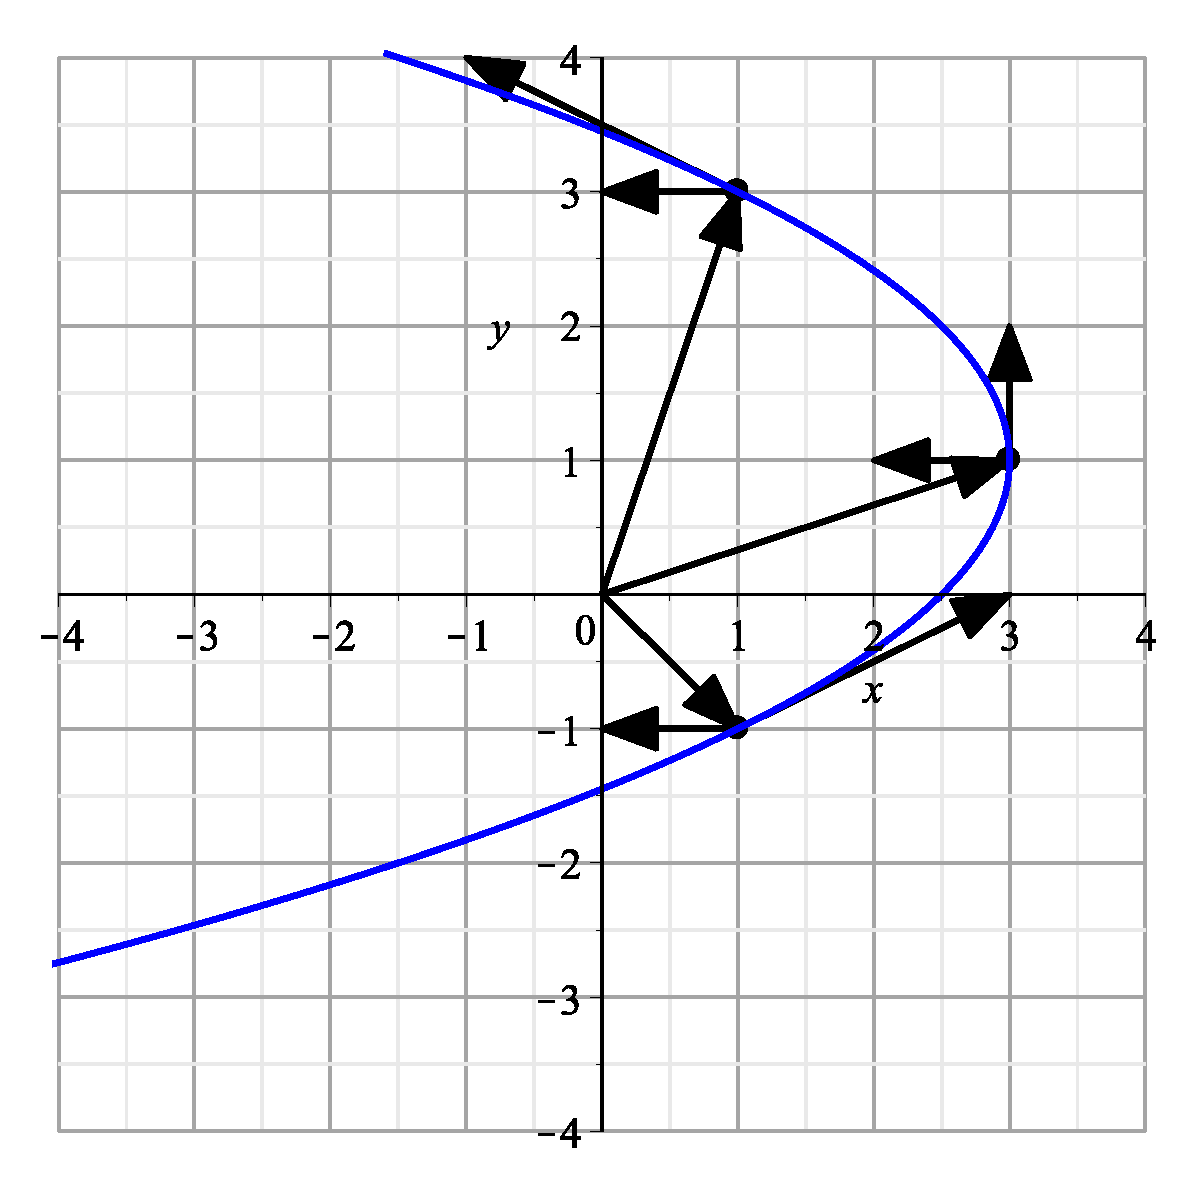
\includegraphics{figures/9_7_8_a.eps}} \ \ \ \  \resizebox{!}{2.5in}{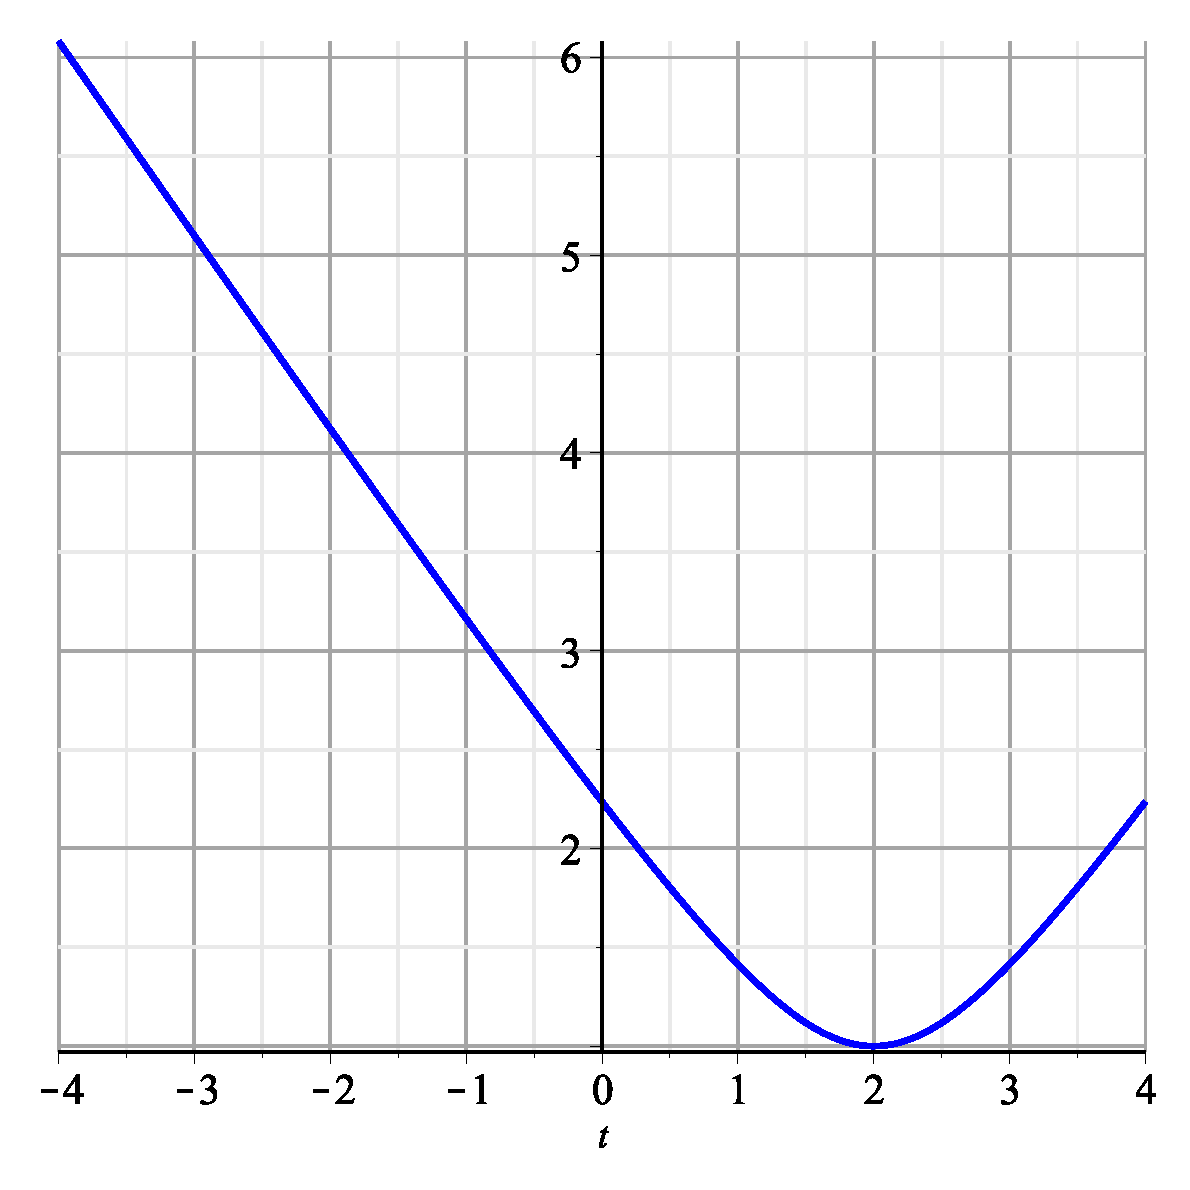
\includegraphics{figures/9_7_8_b.eps}}
\end{center}

\item When $t < 2$ in the position graph, the angle between $\vv$ and $\va$ is larger than $90^{\circ}$. When $t > 2$ in the position graph, the angle between $\vv$ and $\va$ is less than $90^{\circ}$. Note that at the point when $t=2$, the vectors $\vv$ and $\va$ are orthogonal.

	\item Using derivative properties we have 
	\[\frac{d}{dt}(\vv\cdot\vv) = \vv \cdot \frac{d}{dt} \vv + \frac{d}{dt} \vv \cdot \vv = 2(\vv \cdot \va).\]
	So the derivative of the speed is positive when $\vv \cdot \va$ is positive and negative when $\vv \cdot \va$ is negative. In other words, speed is increasing when $\vv \cdot \va$ is positive and decreasing when $\vv \cdot \va$ is negative. When $t < 2$ in the position graph, the angle between $\vv$ and $\va$ is larger than $90^{\circ}$ and so $\vv \cdot \va < 0$. When $t > 2$ in the position graph, the angle between $\vv$ and $\va$ is less than $90^{\circ}$ and so $\vv \cdot \va > 0$. Note that at the point when $t=2$, the vectors $\vv$ and $\va$ are orthogonal.  

\item In general, if $\vr(t) = \langle x(t), y(t) \rangle$, then $\vv(t) = \langle x'(t), y'(t) \rangle$, $\va(t) = \langle x''(t), y''(t) \rangle$, and the speed is $s(t) = \sqrt{(x'(t))^2 + (y'(t))^2}$. Recall that $\comp_{\vv} \va = \frac{\va \cdot \vv}{|\vv|}$, so
\[\frac{d}{dt} s(t) = \frac{x'(t)x''(t) +y'(t)y''(t)}{|\vv|} = \comp_{\vv} \va.\]
 

   \ea

\end{activitySolution}
\aftera


%\begin{activity} \label{A:9.7.9} A {\em central force} is one that
  acts on an object so that the force $\vF$ is parallel to the
  object's position $\vr$.  Since Newton's Second Law says that an
  object's acceleration is proportional to the force exerted on it,
  the acceleration $\va$ of an object moving under a central force
  will be parallel to its position $\vr$.  For instance, the Earth's
  acceleration due to the 
  gravitational force that the sun exerts on the Earth is parallel to
  the Earth's position vector as shown in Figure \ref{F:9.7.sun}.

\begin{figure}[ht]
  \begin{center}
    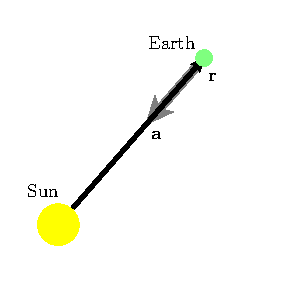
\includegraphics{figures/fig_9_7_sun.eps}
    \caption{A central force.}
    \label{F:9.7.sun}
  \end{center}
\end{figure}

\ba
\item If an object of mass $m$ is moving under a central force, 
  the angular momentum vector is defined to be $\vL=m\vr\times\vv$.
  Assuming the mass is constant, show that the angular momentum is
  constant by showing that
  $$
  \frac{d\vL}{dt} = 0.
  $$

\item Explain why $\vL\cdot\vr = 0$.

\item Explain why we may conclude that the object is constrained to
  lie in the plane passing through the origin and perpendicular to
  $\vL$.





\ea

\end{activity}
\begin{smallhint}

\end{smallhint}
\begin{bighint}

\end{bighint}
\begin{activitySolution}
   \ba
    \item The quantity $\vr(t+h)-\vr(t)$ is a vector quantity, the vector from the terminal point of $\vr(t)$ to the terminal point of $\vr(t+h)$.

    \item The quantity $\frac{\vr(t+h)-\vr(t)}{h}$ is a vector quantity, it is a vector in the direction of $\vr(t+h)-\vr(t)$ that is $\frac{1}{h}$ times as long. 

    \item The vector $\vr(t+h)-\vr(t)$ represents a change in position of the object on the time interval $[t, t+h]$. When we multiply by $\frac{1}{h}$, we can consider this vector  $\frac{\vr(t+h)-\vr(t)}{h}$ as an average change of position, or the average velocity vector of the object on the interval $[t,t+h]$. 

    \item As $h \to 0$, the average velocity vectors $\frac{\vr(t+h)-\vr(t)}{h}$ approach the instantaneous velocity vector. The average velocity vector $\frac{\vr(t+h)-\vr(t)}{h}$ is a direction vector for the secant line to the curve that passes through the terminal points of $\vr(t)$ and $\vr(t+h)$. As we let $h \to 0$, these direction vectors approach a direction vector  
        \[\ds \lim_{h \to 0} \frac{\vr(t+h)-\vr(t)}{h}\]
of the tangent line to the curve at the terminal point of $\vr(t)$. 
    \ea

\end{activitySolution}
\aftera


% To get a flavor for how to verify these properties, consider property
% (4). Let ${\vr(t) = \langle x_r(t), y_r(t), z_r(t) \rangle}$ and
% ${\vs(t) = \langle x_s(t), y_s(t), z_s(t) \rangle}$. Then
% \begin{align*} %\frac{d}{dt}\left( \vr(t) \times \vs(t) \right) &=
% \frac{d}{dt} \big([y_r(t)z_s(t)-y_s(t)z_r(t)] \vi +
% [x_s(t)z_r(t)-x_r(t)z_s(t)] \vj \\ % &\qquad +
% [x_r(t)y_s(t)-x_s(t)y_r(t)] \vk \big) \\ % &=
% \left(\frac{d}{dt}[y_r(t)z_s(t)-y_s(t)z_r(t)]\right) \vi + \left(
% \frac{d}{dt} [x_s(t)z_r(t)-x_r(t)z_s(t)] \right) \vj \\ % &\qquad +
% \left(\frac{d}{dt} [x_r(t)y_s(t)-x_s(t)y_r(t)]\right) \vk \\ % &=
% [(y_r(t)z'_s(t)+y_r'(t)z_s(t))-(y_s(t)z'_r(t)+y_s'(t)z_r(t)] \vi \\ %
% &\qquad + [(x_s(t)z'_r(t)+x'_s(t)z_r(t))-(x_r(t)z'_s(t)+x'_r(t)z_s(t)]
% \vj \\ % &\qquad +
% [(x_r(t)y'_s(t)+x'_r(t)y_s(t))-(x_s(t)y'_r(t)+x'_s(t)y_r(t))] \vk \\ %
% &= \left([y_r'(t)z_s(t)-y_s(t)z'_r(t)]\vi + [x_s(t)z'_r(t) -
% x'_r(t)z_s(t)] \vj + [x'_r(t)y_s(t) - x_s(t)y'_r(t)] \vk \right) \\ %
% &\qquad + \big([y_r(t)z'_s(t)-y_s'(t)z_r(t)] \vi +
% [x'_s(t)z_r(t)-x_r(t)z'_s(t)] \vj \\ % &\qquad +
% [x_r(t)y'_s(t)-x'_s(t)y_r(t)] \vk \big) \\ % &= \vr'(t) \times \vs(t)
% + \vr(t) \times \vs'(t).
% \end{align*} The verification of these properties is left as an
% exercise for the reader.

%\begin{activity} \label{A:9.7.3} Use the properties of differentiation of vector-valued functions to find the following derivatives.
    \ba
    \item $\ds \frac{d}{dt} \sin(t) \langle 2t, t^2, \arctan(t) \rangle$



    \item $\ds \frac{d}{dt} \left(\vr(2^t) \right)$, where $\vr(t) = \langle t+2, \ln(t), 1 \rangle$.



    \ea

\end{activity}
\begin{smallhint}

\end{smallhint}
\begin{bighint}

\end{bighint}
\begin{activitySolution}

\end{activitySolution}
\aftera


\subsection*{Tangent Lines}

One of the most important ideas in first-semester calculus is that a
differentiable function is \emph{locally linear}: that is, when viewed
up close, the curve generated by a differentiable function looks very
much like a line.  Indeed, when we zoom in sufficiently far on a
particular point, the curve looks indistinguishable from its tangent
line.

In the same way, we expect that a smooth curve in 3-space will be
locally linear.  In the following activity, we investigate how to find
the tangent line to such a curve.  Recall from our work in
Section~\ref{S:9.5.Lines_Planes} that the vector equation of a line that
passes through the point at the tip of the vector $\vL_0 = \langle
x_0, y_0, z_0 \rangle$ in the direction of the vector $\vu = \langle
a, b, c \rangle$ can be written as
$$\vL(t) = \vL_0 + t \vu.$$
In parametric form, the line $\vL$ is given by
$$x(t) = x_0 + at, \ \ y(t) = y_0 + bt, \ \ z(t) = z_0 + ct.$$

\newpage

\begin{activity} \label{A:9.7.4} Let
\[\vr(t) = \cos(t) \vi - \sin(t) \vj + t \vk.\footnote{You can sketch the graph with Wolfram Alpha, the applet at \url{http://gvsu.edu/s/LR}, or some other appropriate technology.}\]
    \ba
    
    \item Determine the coordinates of the point on the curve traced out by $\vr(t)$ when $t = \pi$.
    
    \item Find a direction vector for the line tangent to the graph of $\vr$ at the point where $t=\pi$.

    \item Find the parametric equations of the line tangent to the graph of $\vr$ when $t=\pi$.

    \item Sketch a plot of the curve $\vr(t)$ and its tangent line near the point where $t = \pi$.  In addition, include a sketch of $\vr'(\pi)$.  What is the important role of $\vr'(\pi)$ in this activity?

    \ea

\end{activity}
\begin{smallhint}

\end{smallhint}
\begin{bighint}

\end{bighint}
\begin{activitySolution}
    \ba
    \item Since
    \[\vr(\pi) = \cos(\pi) \vi - \sin(\pi) \vj + \pi \vk = -\vi + \pi \vk,\]
the point on the curve traced out by $\vr(t)$ when $t = \pi$ is $(-1,0,\pi)$. 
    \item The derivative 
\[\vr'(\pi) = -\sin(\pi)\vi - \cos(\pi)\vj + \vk = \vj + \vk\]
is a direction vector for the line tangent to the graph of $\vr$ at the point where $t=\pi$.
    \item Using the point and the direction vector found in (a) and (b), the parametric equations of the line tangent to the graph of $\vr$ when $t=\pi$ are
\[x(t) = -1, \ \ \ y(t) = t, \ \ \ z(t) = \pi+t.\]
    \item The sketch below shows the curve $\vr(t)$ and a direction vector $\vr'(\pi)$ for the tangent line to the curve at $t=\pi$. 
%\begin{figure}[ht]
\begin{center}
\resizebox{!}{2.0in}{\includegraphics{figures/9_7_Act29_d_sol}}
%\caption{The distance formula in $\R^3$.}
%\label{F:9.1.Distance_3D}
\end{center}
%\end{figure}

    \ea
\end{activitySolution}
\aftera


We see that our work in Activity~\ref{A:9.7.4} can be generalized.
Given a differentiable vector-valued function $\vr(t)$, the tangent
line to the curve at the input value $a$ is given by
\begin{equation} \label{E:TanLineVecFxn} \vL(t) = \vr(a) + t \vr'(a).
\end{equation} Here we see that because the tangent line is determined
entirely by a given point and direction, the point is provided by the
function $\vr(t)$, evaluated at $t = a$, while the direction is
provided by the derivative, $\vr'(t)$, again evaluated at $t = a$.
Note how analogous the formula for $\vL(t)$ is to the tangent line
approximation from single-variable calculus: in that context, for a
given function $y = f(x)$ at a value $x = a$, we found that the
tangent line can be expressed by the linear function $y = L(x)$ whose
formula is
$$L(x) = f(a) + f'(a)(x-a).$$
Equation~\eqref{E:TanLineVecFxn} for the tangent line $\vL(t)$ to the
vector-valued function $\vr(t)$ is nearly identical.  Indeed, because
there are multiple parameterizations for a single line, it is even
possible\footnote{In Equation~\eqref{E:TanLineVecFxn}, $\vL(0) =
\vr(a)$, so the line's parameterization ``starts'' at $t = 0$.  When
we write the parameterization in the form of
Equation~\eqref{E:TanLineVecFxn2}, $\vL(a) = \vr(a)$, so the line's
parameterization ``starts'' at $t = a$.} to write the parameterization
as
\begin{equation} \label{E:TanLineVecFxn2} \vL(t) = \vr(a) + (t-a)
\vr'(a).
\end{equation}

As we will learn more in Chapter 10, a smooth surface in 3-space is
also locally linear. That means that the surface will look like a
plane, which we call its {\em tangent plane}, as we zoom in on the
graph.  It is possible to use tangent lines to traces of the surface
to generate a formula for the tangent plane; see
Exercise~\ref{Ez:9.7.3} at the end of this section for more details.

%\begin{activity} \label{A:9.7.5} In this activity we determine the equation of a plane tangent to the surface defined by $f(x,y) = x^2+y^2$ at the point $(3,4,5)$.
    \ba
    \item Find a parameterization for the $x=3$ trace to $f$. What is a direction vector for the line tangent to this trace at the point $(3,4,5)$?



    \item  Find a parameterization for the $y=4$ trace to $f$. What is a direction vector for the line tangent to this trace at the point $(3,4,5)$?



    \item The direction vectors in parts (a) and (b) form a plane containing the point $(3,4,5)$. What is a normal vector for this plane? Find the equation of this plane. Use appropriate technology to draw the graph of $f$ and the plane you determined on the same set of axes. What do you notice? (This plane is the tangent plane to $f$ at the point $(3,4,5)$. We will discuss tangent planes in more detail in a later section.)



    \ea

\end{activity}
\begin{smallhint}

\end{smallhint}
\begin{bighint}

\end{bighint}
\begin{activitySolution}

\end{activitySolution}
\aftera




\subsection*{Integrating a Vector-Valued Function}

Recall from single variable calculus that an antiderivative of a
function $f$ of the independent variable $x$ is a function $F$ that
satisfies $F'(x) = f(x)$. We then defined the indefinite integral
$\int f(x) \ dx$ to be the general antiderivative of $f$.  Recall that
the general antiderivative includes an added constant $C$ in order to
indicate that the general antiderivative is in fact an entire family
of functions. We can do the similar work with vector-valued functions.

\vspace*{5pt} \nin \framebox{\hspace*{3 pt}
\parbox{6.25 in}{\begin{definition} An
\textbf{antiderivative}\index{vector-valued function!antiderivative}
of a vector-valued function $\vr$ is a vector-valued function $\vR$
such that
\[\vR'(t) = \vr(t).\]

The \textbf{indefinite integral}\index{vector-valued
function!indefinite integral} $\int \vr(t) \ dt$ of a vector-valued
function $\vr$ is the general antiderivative of $\vr$ and represents the
collection of all antiderivatives of $\vr$. \end{definition} }
\hspace*{3 pt}} \vspace*{5pt}

The same reasoning that allows us to differentiate a vector-valued
function componentwise applies to integrating as well. Recall that the
integral of a sum is the sum of the integrals and also that we can
remove constant factors from integrals. So, given ${\vr(t) = x(t) \vi
+ y(t) \vj + z(t) \vk}$, it follows that we can integrate
componentwise. Expressed more formally,

\vspace*{5pt} \nin \framebox{\hspace*{3 pt}
\parbox{6.25 in}{If $\vr(t) = x(t) \vi + y(t) \vj + z(t) \vk$, then
\[\int \vr(t) \ dt = \left(\int x(t) \ dt\right) \vi + \left( \int
y(t) \ dt \right) \vj + \left(\int z(t) \ dt\right) \vk.\] }
\hspace*{3 pt}} \vspace*{5pt}

%\input{activities/9.7.Act6}

In light of being able to integrate and differentiate componentwise
with vector-valued functions, we can solve many problems that are
analogous to those we encountered in single-variable calculus.  For
instance, recall problems where we were given an object moving along
an axis with velocity function $v(t)$ and an initial position $s(0)$.
In that context, we were able to differentiate $v$ in order to find
acceleration, and integrate $v$ and use the initial condition in order
to find the position function $s$.  In the following activity, we
explore similar ideas with vector-valued functions.

\begin{activity} \label{A:9.7.7} 
Suppose a moving object in space has its velocity given by
\[\vv(t) = (-2\sin(2t)) \vi + (2 \cos(t)) \vj + \left(1 - \frac{1}{1+t}\right) \vk.\]
A graph of the position of the object for times $t$ in $[-0.5,3]$ is shown in Figure \ref{F:9.7.VVD_Example}.  Suppose further that the object is at the point $(1.5,-1,0)$ at time $t=0$. 
	\ba
	\item Determine $\va(t)$, the acceleration of the object at time $t$.

	\item Determine $\vr(t)$, position of the object at time $t$.

	\item Compute and sketch the position, velocity, and acceleration vectors of the object at time $t=1$, using Figure~\ref{F:9.7.VVD_Example}.
	
	\item Finally, determine the vector equation for the tangent line, $\vL(t)$, that is tangent to the position curve at $t = 1$.

	\ea
\begin{figure}[ht]
\begin{center}
%\scalebox{0.5}{\includegraphics{9_7_VVD_Example}}
\includegraphics{figures/fig_9_7_activity.eps}
\caption{The position graph for the function in Activity~\ref{A:9.7.7}.}
\label{F:9.7.VVD_Example}
\end{center}
\end{figure}

\end{activity}
\begin{smallhint}

\end{smallhint}
\begin{bighint}

\end{bighint}
\begin{activitySolution}
	\ba
	\item Since acceleration is the derivative of the velocity we have 
\[\va(t) = \vv'(t) = -4\cos(2t)\vi -2\sin(t) \vj + \left(\frac{1}{(1+t)^2}\right) \vk.\]

	\item The position of the object is an antiderivative of the velocity, so 
\[\vr(t) = \int \vv(t) \, dt = \cos(2t) \vi + 2\sin(t) \vj + \left( t - \ln|1+t| \right) \vk + \vC\]
for some constant $\vC$. Since $\vr(0) = \langle 1.5, -1, 0 \rangle$, we have 
\[\langle 1.5, -1, 0 \rangle = \vr(0) = \langle 1, 0, 0 \rangle + \vC\]
and so $\vC = \langle 0.5, -1, 0 \rangle$. Therefore,
\[\vr(t) = (\cos(2t)+0.5) \vi + (2\sin(t)-1) \vj + \left( t - \ln|1+t| \right) \vk.\]
	\item The position $\vr(1) = (\cos(2)+1) \vi + (2\sin(1)-1) \vj + (1-ln(2)) \vk$, velocity $\vv(1) = (-2\sin(2)) \vi + (2\cos(1)) \vj + \left(\frac{1}{2}\right) \vk$, and acceleration vector $\va(1) = (-4\cos(2)) \vi - (2\sin(1)) \vj + \left(\frac{1}{4}\right) \vk$ of the object at time $t=1$ are shown below. 
%\begin{figure}[ht]
\begin{center}
\resizebox{!}{2.0in}{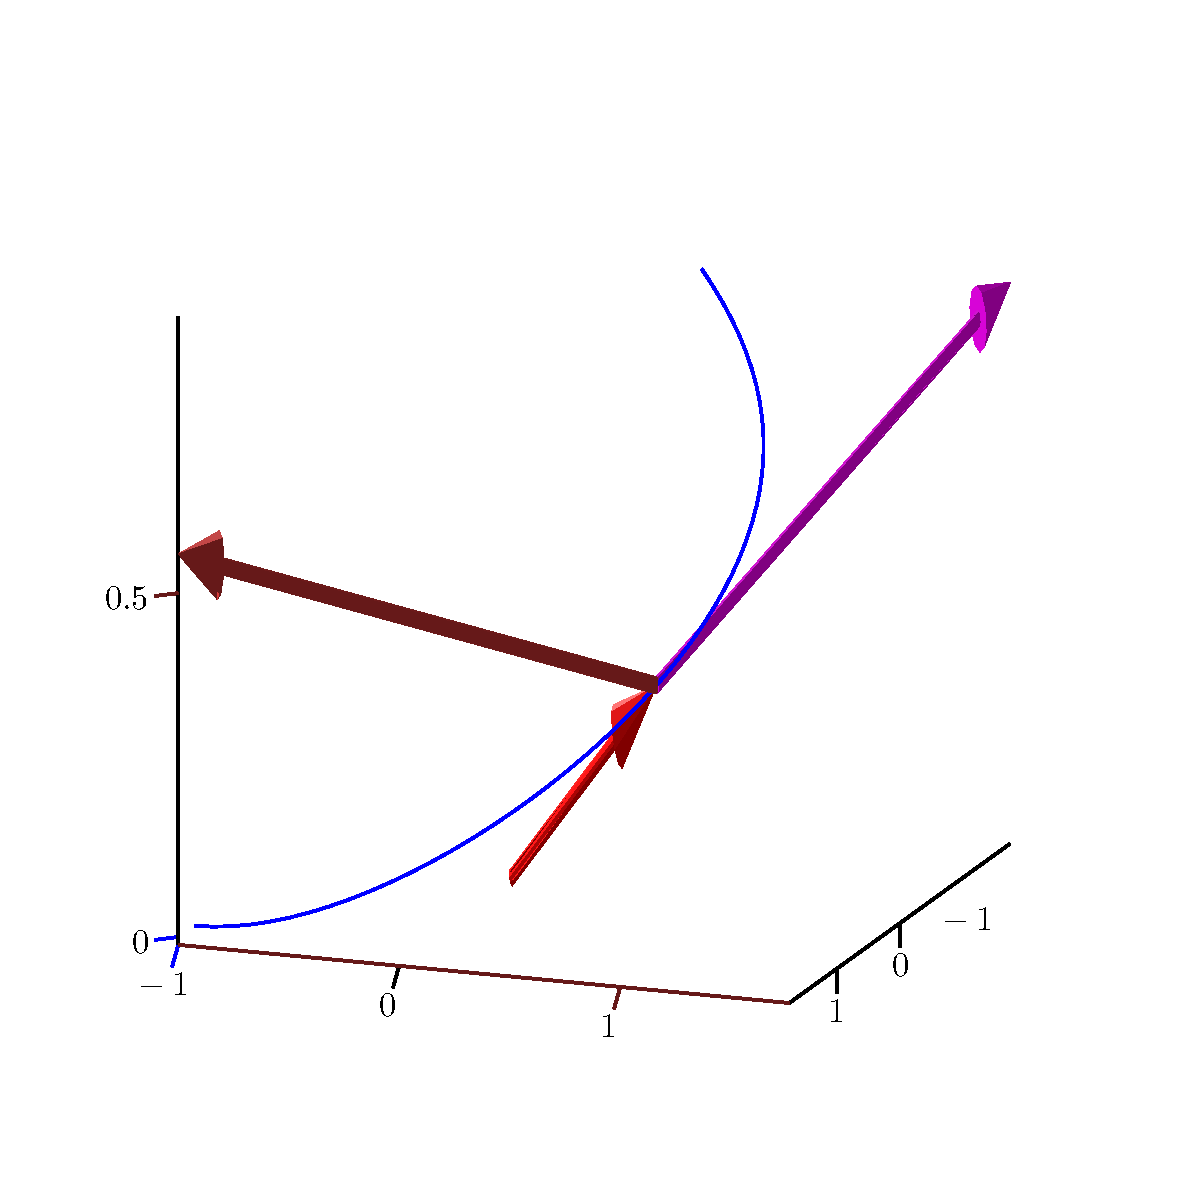
\includegraphics{figures/9_7_Act30_c_sol}}
%\caption{The distance formula in $\R^3$.}
%\label{F:9.1.Distance_3D}
\end{center}
%\end{figure}	
	\item The vector $\vv(1)$ is a direction vector for $\vL(t)$ and so
\[\vL(t) = \vr(1) + t\vv(1) = \langle \cos(2)+1, 2\sin(1)-1, 1-\ln(2) \rangle + t \left\langle -2\sin(2), 2\cos(1), + \frac{1}{2} \right\rangle.\]


	\ea
\end{activitySolution}
\aftera



\subsection*{Projectile Motion}

%\begin{pa} \label{PA:9.7.2} When computers first came out, there was a QBasic game, Gorillas, in which gorillas threw banana grenades at each other attempting to blow each other up.\footnote{A on-line version can be found at \url{http://www.online-games-zone.com/pages/classic/gorillas.php}. No endorsement of this site or the advertisements is implied.} Typically, a player uses trial and error to determine the correct velocity and launch angle to destroy his/her opponent. Play a few rounds of this game and come up with a strategy to win the game.

\end{pa} \afterpa 

Any time that an object is launched into the air with a given velocity
and launch angle, the path the object travels is determined almost
exclusively by the force of gravity.  Whether in sports such as
archery or shotput, in military applications with artillery, or in
important fields like firefighting, it is important to be able to know
when and where a launched projectile will land.  We can use our
knowledge of vector-valued functions in order to completely determine
the path traveled by an object that is launched from a given position
at a given angle from the horizontal with a given initial velocity.

\begin{figure}[ht]
\begin{center} 
%\resizebox{!}{1.0in}{\includegraphics{9_7_Motion}}
\includegraphics{figures/fig_9_7_projectile.eps}
\caption{Projectile motion.}
\label{F:9.7.Motion}
\end{center}
\end{figure}

Assume we fire a projectile from a launcher and the only force acting
on the fired object is the force of gravity pulling down on the
object.  That is, we assume no effect due to spin, wind, or air
resistance.  With these assumptions, the motion of the object will be
planar, so we can also assume that the motion occurs in
two-dimensional space. Suppose we launch the object from an initial
position $(x_0, y_0)$ at an angle $\theta$ with the positive $x$-axis
as illustrated in Figure \ref{F:9.7.Motion}, and that we fire the
object with an initial speed of $v_0 = |\vv(0)|$, where $\vv(t)$ is
the velocity vector of the object at time $t$.  Assume $g$ is the
positive constant acceleration force due to gravity, which acts to
pull the fired object toward the ground (in the negative $y$
direction). Note particularly that there is no external force acting
on the object to move it in the $x$ direction.

We first observe that since gravity only acts in the downward
direction and that the acceleration due to gravity is constant,
the acceleration vector is $\langle 0, -g
\rangle$.  That is, $\va(t) = \langle 0, -g \rangle$.  We may use this
fact about acceleration, together with the initial position and
initial velocity in order to fully determine the position function
$\vr(t)$ of the object at time $t$.  In Exercise~\ref{Ez:9.7.5}, you
can work through the details to show that the following general
formula holds.

%\begin{activity} \label{A:9.7.8} The left side of figure
  \ref{F:9.7.space.curve} shows the curve described by the
  vector-valued function
  $$\vr(t) = \left\langle 2t-\frac12 t^2 + 1,
        t-1\right\rangle.$$

\begin{figure}[ht]
  \begin{center}
    \includegraphics{figures/fig_9_7_space_curve.eps}
    \hspace*{20pt}
    \includegraphics{figures/fig_9_7_speed_graph.eps}
    \caption{The curve $\vr(t) = \left\langle 2t-\frac12 t^2 + 1,
        t-1\right\rangle$ and its speed.}
    \label{F:9.7.space.curve}
  \end{center}
\end{figure}

\ba
\item Find the object's velocity $\vv(t)$.

\item Find the object's acceleration $\va(t)$.

\item Indicate on the left of Figure \ref{F:9.7.space.curve} the object's
  position, velocity and acceleration at the times $t=0, 2, 4$.  Draw
  the velocity and acceleration vectors with their tails placed at the
  object's position.

\item Recall that the speed is $|\vv| = \sqrt{\vv\cdot\vv}$. Find the object's speed and graph it as a function of time $t$ on the right of Figure \ref{F:9.7.space.curve}.  When is the
  object's speed the slowest?  When is the speed increasing?  When it
  is decreasing?

\item What seems to be true about the angle between $\vv$ and $\va$ when the speed
  is at a minimum?  What is the angle between $\vv$ and $\va$
  when the speed is increasing?  when the speed is decreasing?

\item   Since the square root is an increasing function, we see that the speed
  increases precisely when $\vv\cdot\vv$ is increasing.  Use the
  product rule for the dot product to express
  $\frac{d}{dt}(\vv\cdot\vv)$ in terms of the velocity $\vv$ and
  acceleration $\va$.  Use this to explain why the speed is increasing
  when $\vv\cdot\va > 0$ and decreasing when
  $\vv\cdot\va < 0$. Compare this to part (d). 

\item Show that the speed's rate of change is
  $$
  \frac{d}{dt}|\vv(t)| = \comp_{\vv} \va.
  $$





\ea

\end{activity}
\begin{smallhint}

\end{smallhint}
\begin{bighint}

\end{bighint}
\begin{activitySolution}
   \ba
    \item Velocity is the derivative of position, so
\[\vv(t) = \vr'(t)= \langle 2-t, 1 \rangle.\]


    \item Acceleration is the derivative of velocity, so
\[\va(t) = \vv'(t)= \langle -1, 0 \rangle.\]

    \item Notice that $\vr(0) = \langle 1,-1 \rangle$, $\vr(2) = \langle 2,1 \rangle$, and $\vr(4) = \langle 0,3 \rangle$. The vectors at each point are shown in the figure below at left. 


    \item Speed is the magnitude of the velocity, so the speed of the object at time $t$ is
\[s(t) = \sqrt{(2-t)^2+1}.\]
The speed of the object is at its least when $t=2$. The speed is increasing on the interval $(2,4)$ and decreasing on the interval $(-4,2)$.  
\begin{center}
\resizebox{!}{2.5in}{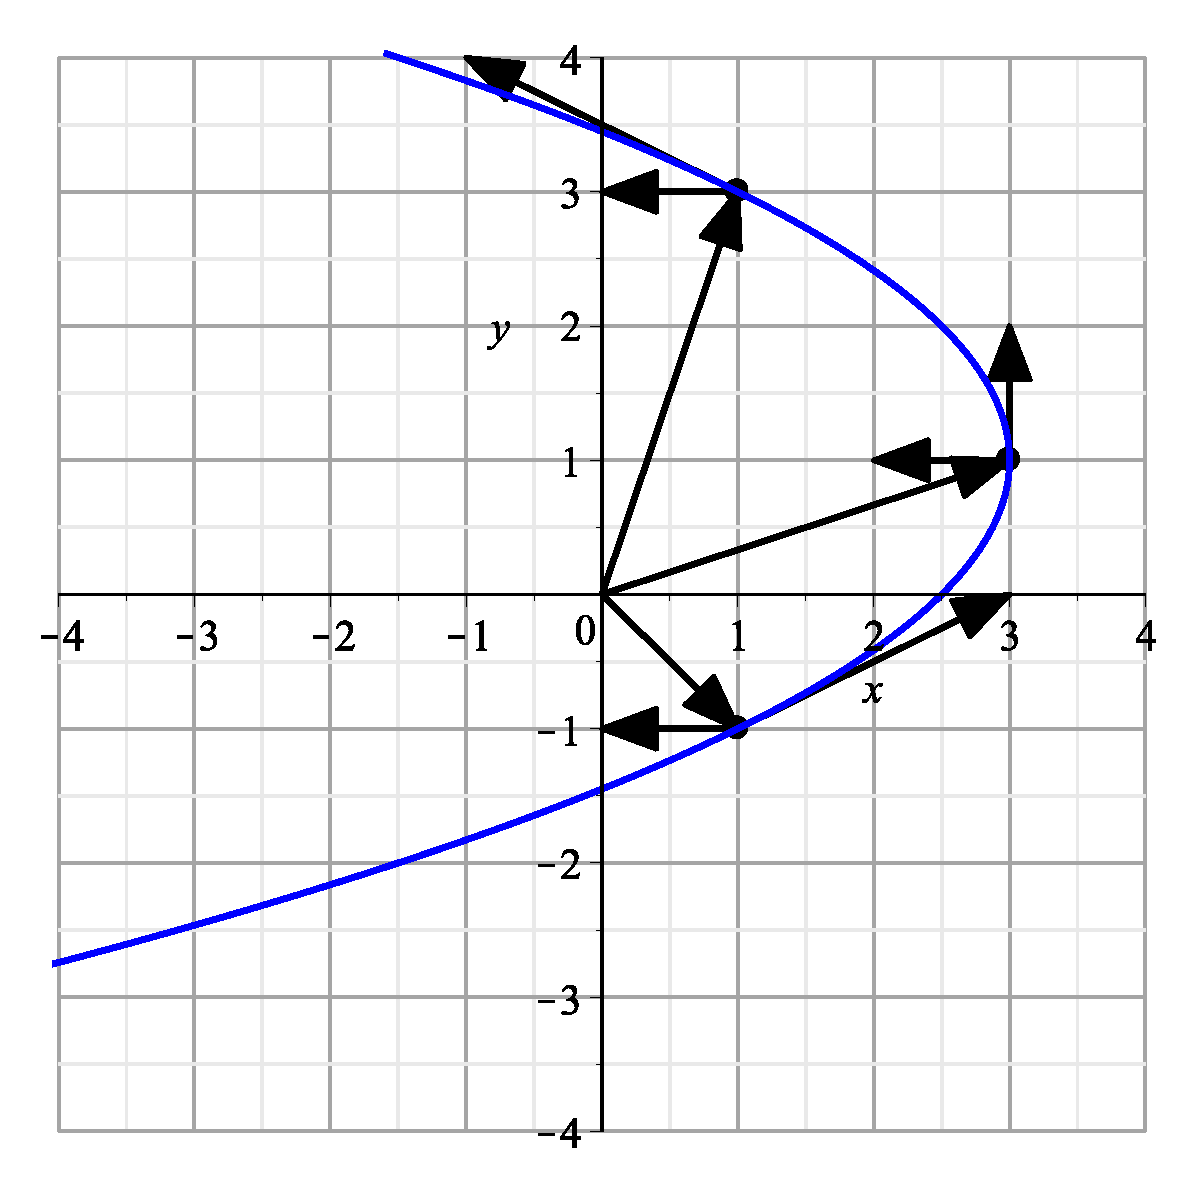
\includegraphics{figures/9_7_8_a.eps}} \ \ \ \  \resizebox{!}{2.5in}{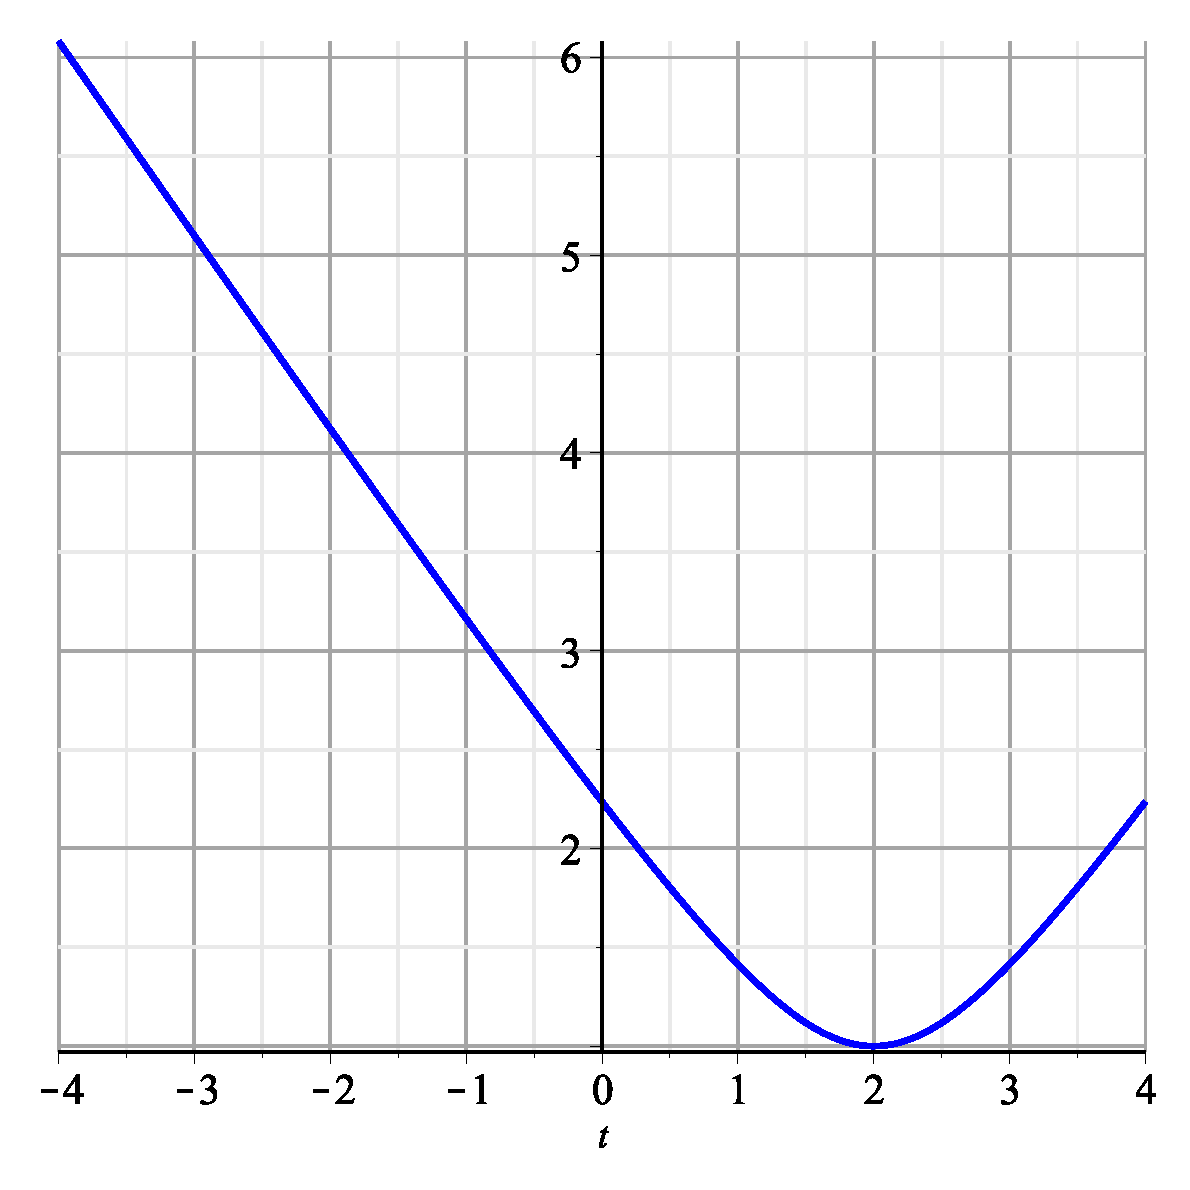
\includegraphics{figures/9_7_8_b.eps}}
\end{center}

\item When $t < 2$ in the position graph, the angle between $\vv$ and $\va$ is larger than $90^{\circ}$. When $t > 2$ in the position graph, the angle between $\vv$ and $\va$ is less than $90^{\circ}$. Note that at the point when $t=2$, the vectors $\vv$ and $\va$ are orthogonal.

	\item Using derivative properties we have 
	\[\frac{d}{dt}(\vv\cdot\vv) = \vv \cdot \frac{d}{dt} \vv + \frac{d}{dt} \vv \cdot \vv = 2(\vv \cdot \va).\]
	So the derivative of the speed is positive when $\vv \cdot \va$ is positive and negative when $\vv \cdot \va$ is negative. In other words, speed is increasing when $\vv \cdot \va$ is positive and decreasing when $\vv \cdot \va$ is negative. When $t < 2$ in the position graph, the angle between $\vv$ and $\va$ is larger than $90^{\circ}$ and so $\vv \cdot \va < 0$. When $t > 2$ in the position graph, the angle between $\vv$ and $\va$ is less than $90^{\circ}$ and so $\vv \cdot \va > 0$. Note that at the point when $t=2$, the vectors $\vv$ and $\va$ are orthogonal.  

\item In general, if $\vr(t) = \langle x(t), y(t) \rangle$, then $\vv(t) = \langle x'(t), y'(t) \rangle$, $\va(t) = \langle x''(t), y''(t) \rangle$, and the speed is $s(t) = \sqrt{(x'(t))^2 + (y'(t))^2}$. Recall that $\comp_{\vv} \va = \frac{\va \cdot \vv}{|\vv|}$, so
\[\frac{d}{dt} s(t) = \frac{x'(t)x''(t) +y'(t)y''(t)}{|\vv|} = \comp_{\vv} \va.\]
 

   \ea

\end{activitySolution}
\aftera
 
% Ultimately, we want to find the position
% of the object as it travels through space so that we can determine
% what initial velocity and launch angle to provide so that we hit our
% target.  %\begin{activity} \label{A:9.7.9} A {\em central force} is one that
  acts on an object so that the force $\vF$ is parallel to the
  object's position $\vr$.  Since Newton's Second Law says that an
  object's acceleration is proportional to the force exerted on it,
  the acceleration $\va$ of an object moving under a central force
  will be parallel to its position $\vr$.  For instance, the Earth's
  acceleration due to the 
  gravitational force that the sun exerts on the Earth is parallel to
  the Earth's position vector as shown in Figure \ref{F:9.7.sun}.

\begin{figure}[ht]
  \begin{center}
    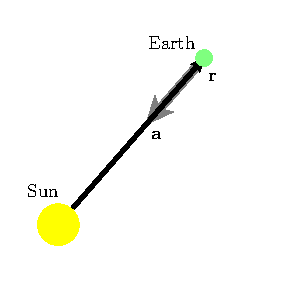
\includegraphics{figures/fig_9_7_sun.eps}
    \caption{A central force.}
    \label{F:9.7.sun}
  \end{center}
\end{figure}

\ba
\item If an object of mass $m$ is moving under a central force, 
  the angular momentum vector is defined to be $\vL=m\vr\times\vv$.
  Assuming the mass is constant, show that the angular momentum is
  constant by showing that
  $$
  \frac{d\vL}{dt} = 0.
  $$

\item Explain why $\vL\cdot\vr = 0$.

\item Explain why we may conclude that the object is constrained to
  lie in the plane passing through the origin and perpendicular to
  $\vL$.





\ea

\end{activity}
\begin{smallhint}

\end{smallhint}
\begin{bighint}

\end{bighint}
\begin{activitySolution}
   \ba
    \item The quantity $\vr(t+h)-\vr(t)$ is a vector quantity, the vector from the terminal point of $\vr(t)$ to the terminal point of $\vr(t+h)$.

    \item The quantity $\frac{\vr(t+h)-\vr(t)}{h}$ is a vector quantity, it is a vector in the direction of $\vr(t+h)-\vr(t)$ that is $\frac{1}{h}$ times as long. 

    \item The vector $\vr(t+h)-\vr(t)$ represents a change in position of the object on the time interval $[t, t+h]$. When we multiply by $\frac{1}{h}$, we can consider this vector  $\frac{\vr(t+h)-\vr(t)}{h}$ as an average change of position, or the average velocity vector of the object on the interval $[t,t+h]$. 

    \item As $h \to 0$, the average velocity vectors $\frac{\vr(t+h)-\vr(t)}{h}$ approach the instantaneous velocity vector. The average velocity vector $\frac{\vr(t+h)-\vr(t)}{h}$ is a direction vector for the secant line to the curve that passes through the terminal points of $\vr(t)$ and $\vr(t+h)$. As we let $h \to 0$, these direction vectors approach a direction vector  
        \[\ds \lim_{h \to 0} \frac{\vr(t+h)-\vr(t)}{h}\]
of the tangent line to the curve at the terminal point of $\vr(t)$. 
    \ea

\end{activitySolution}
\aftera
 %Now we can find the position
% vector for the object at any time.  %\begin{activity} \label{A:9.7.10} Let $\vv(t)$ be the velocity vector found in Activity \ref{A:9.7.9}.
\ba
    \item Find all possible position vectors for the velocity vector $\vv(t)$.



\begin{comment}

If $\vr$ is the vector-valued function that gives the position of the object at time $t$, then
\[\vr(t) = \int \vv(t) \ dt = \left\langle v_0 \cos(\theta)t, -g\frac{t^2}{2} + v_0 \sin(\theta)t \right\rangle + \vk,\]
where $\vk$ is some constant vector.

\end{comment}

    \item Let $\vr(t)$ denote the position vector function for our projectile. Use the fact that the object is fired from the position $(x_0, y_0)$ to explain why
\[\vr(t) = \left\langle v_0 \cos(\theta)t + x_0, -g\frac{t^2}{2} + v_0 \sin(\theta)t + y_0 \right\rangle.\]



\begin{comment}

Now $\vr(0) = \langle x_0, y_0 \rangle$, so we have
\[\langle x_0, y_0 \rangle =  \langle v_0 \cos(\theta)(0), -g\frac{0^2}{2} + v_0 \sin(\theta)(0) \rangle + \vk\]
and
\[\vk = \langle x_0, y_0 \rangle.\]
We conclude that
\[\vr(t) = \langle v_0 \cos(\theta)t + x_0, -g\frac{t^2}{2} + v_0 \sin(\theta)t + y_0 \rangle.\]

\end{comment}

    \ea

\end{activity}
\begin{smallhint}

\end{smallhint}
\begin{bighint}

\end{bighint}
\begin{activitySolution}

\end{activitySolution}
\aftera
 %We
% summarize the result of Activities \ref{A:9.7.7} through
% \ref{A:9.7.9}.

\vspace*{5pt} \nin \framebox{\hspace*{3 pt}
\parbox{6.25 in}{If an object is launched from a point $(x_0,y_0)$
with initial velocity $v_0$ at an angle $\theta$ with the horizontal,
then the position of the object at time $t$ is given by
\[\vr(t) = \left\langle v_0 \cos(\theta)t + x_0, -\frac{g}{2}t^2 + v_0
\sin(\theta)t + y_0 \right\rangle.\] This assumes that the only force
acting on the object is the acceleration $g$ due to
gravity.\index{projectile motion!parametric equations} } \hspace*{3
pt}} \vspace*{5pt}

%\begin{activity} \label{A:9.7.11} Suppose our gorilla is perched on a building at a height of 300 feet, and her opponent is at the top of a building 500 feet away at a height of 200 feet. Use $g = 32$ feet per second per second.
    \ba
    \item If our gorilla throws a banana with initial speed of 85 feet per second with a launch angle of $60^{\circ}$ (assuming no buildings are in the way), will the banana hit her opponent?



    \item Is it possible for our gorilla to hit her opponent with the banana if she can provide an initial speed for her banana of 85 feet per second. If yes, at what angle should she release her banana? If no, why not?



    \ea

\end{activity}
\begin{smallhint}

\end{smallhint}
\begin{bighint}

\end{bighint}
\begin{activitySolution}

\end{activitySolution}
\aftera

%\clearpage

\begin{summary}
\item If $\vr$ is a vector-valued function, then the derivative of
$\vr$ is defined by
\[ \vr'(t) = \lim_{h \to 0} \frac{\vr(t+h)-\vr(t)}{h}\] for those
values of $t$ at which the limit exists, and is computed componentwise
by the formula
\[ \vr'(t) = x'(t) \vi + y'(t) \vj + z'(t) \vk \] for those values of
$t$ at which $x$, $y$, and $z$ are differentiable, where $\vr(t) =
x(t) \vi + y(t) \vj + z(t) \vk$.

\item The derivative $\vr'(t)$ of the vector-valued function $\vr$
tells us the instantaneous rate of change of $\vr$ with respect to
time, $t$, which can be interpreted as a direction vector for the line
tangent to the graph of $\vr$ at the point $\vr(t)$, or also as the
instantaneous velocity of an object traveling along the graph defined
by $\vr(t)$ at time $t$.
 
\item An antiderivative of $\vr$ is a vector-valued function $\vR$
such that $\vR'(t) = \vr(t)$.  The indefinite integral $\int \vr(t) \
dt$ of a vector-valued function $\vr$ is the general antiderivative of
$\vr$ (which is a collection of all of the antiderivatives of $\vr$,
with any two antiderivatives differing by at most a constant vector).
Moreover, if $\vr(t) = x(t) \vi + y(t) \vj + z(t) \vk$, then
\[\int \vr(t) \ dt = \left(\int x(t) \ dt\right) \vi + \left( \int
y(t) \ dt \right) \vj + \left(\int z(t) \ dt\right) \vk.\]

\item If an object is launched from a point $(x_0,y_0)$ with initial
velocity $v_0$ at an angle $\theta$ with the horizontal, then the
position of the object at time $t$ is given by
\[\vr(t) = \left\langle v_0 \cos(\theta)t + x_0, -\frac{g}{2}t^2 + v_0
\sin(\theta)t + y_0 \right\rangle,\] provided that that the only force
acting on the object is the acceleration $g$ due to gravity.
\end{summary}


\nin \hrulefill

\newpage

\begin{exercises} 

\item \label{Ez:9.7.1}    Compute the derivative of each of the following functions in two different ways:  (1) use the rules provided in the theorem stated just after Activity~\ref{A:9.7.2}, and (2) rewrite each given function so that it is stated as a single function (either a scalar function or a vector-valued function with three components), and differentiate component-wise.  Compare your answers to ensure that they are the same.
    \ba
    \item $\ds \vr(t) = \sin(t) \langle 2t, t^2, \arctan(t) \rangle$

    \item $\ds \vs(t) = \vr(2^t)$, where $\vr(t) = \langle t+2, \ln(t), 1 \rangle$.
    
    \item $\ds \vr(t) = \langle \cos(t), \sin(t), t \rangle \cdot \langle -\sin(t), \cos(t), 1 \rangle$
    
    \item $\ds \vr(t) = \langle \cos(t), \sin(t), t \rangle \times \langle -\sin(t), \cos(t), 1 \rangle$
     
    \ea

\begin{exerciseSolution}
    \ba
    \item First we use part 2 of the theorem to find that 
\[\vr'(t) = \sin(t) \left\langle 2, 2t, \frac{1}{1+t^2} \right\rangle + \cos(t) \langle 2t, t^2, \arctan(t) \rangle.\]
Next we write $\vr(t)$ as a vector-valued function with three components:
\[\vr(t) = \langle 2t \sin(t), t^2 \sin(t), \arctan(t) \sin(t) \rangle.\]
Then we differentiate component-wise to obtain
\[\frac{d}{dt} \vr(t)  = \left\langle 2\sin(t) + 2t \cos(t), 2t \sin(t) + t^2 \cos(t), \frac{1}{1+t^2} \sin(t) + \arctan(t) \cos(t) \right\rangle.\]

    \item First we use part 5 of the theorem to calculate
\[\vs'(t) = \vr'(2^t)(2^t \ln(2)) = 2^t \ln(2) \left\langle 1, \frac{1}{2^t}, 0 \right\rangle.\]
Next we write $\vs(t)$ as a vector-valued function with three components and differentiate component-wise to obtain
\[\frac{d}{dt} \langle 2^t+2, \ln(2^t), 1 \rangle = \left\langle 2^t \ln(2), \ln(2), 0 \right\rangle.\]
    
    \item First we use part 3 of the theorem to calculate
\[\vr'(t) = \langle -\sin(t), \cos(t), 1 \rangle \cdot \langle -\sin(t), \cos(t), 1 \rangle + \langle \cos(t), \sin(t), t \rangle \cdot \langle -\cos(t), -\sin(t), 0 \rangle.\]
Next we write $\vr(t)$ as a vector-valued function with three components and differentiate component-wise to obtain
\[\frac{d}{dt} \langle -\cos(t) \sin(t), \sin(t) \cos(t), t \rangle = \langle -(\cos^2(t)-\sin^2(t)), \cos^2(t)-\sin^2(t), 1 \rangle.\]
    
    \item First we use part 4 of the theorem and see that 
\[\vr'(t) = \langle -\sin(t), \cos(t), 1 \rangle \times \langle -\sin(t), \cos(t), 1 \rangle + \langle \cos(t), \sin(t), t \rangle \times \langle -\cos(t), -\sin(t), 0 \rangle = \langle t \sin(t), -t\cos(t), 0 \rangle.\]
Next we write $\vr(t)$ as a vector-valued function with three components and differentiate component-wise to obtain
\begin{align*}
\frac{d}{dt} \langle \sin(t)-t\cos(t), -\cos(t)-t\sin(t), 1 \rangle &= \langle \cos(t) - (\cos(t)-t\sin(t)), \sin(t)-(\sin(t)+t\cos(t)), 0 \rangle \\
	&= \langle t \sin(t), -t\cos(t), 0 \rangle.
\end{align*}
     
    \ea
\end{exerciseSolution}


\item \label{Ez:9.7.2}   Consider the two vector-valued functions given by 
$$\vr(t) = \left\langle t + 1, \cos\left(\frac{\pi}{2} t\right), \frac{1}{1+t} \right\rangle$$
and
$$\vw(s) = \left\langle s^2, \sin\left(\frac{\pi}{2}s\right), s \right\rangle.$$ 

%\begin{figure}[h]
%\begin{center}
 %\includegraphics{figures/1_1_Ez1.eps}
 %\caption{A bungee jumper's height function.} \label{F:1.1.Ez1}
%\end{center}
%\end{figure}

\ba

	\item Determine the point of intersection of the curves generated by $\vr(t)$ and $\vw(s)$.  To do so, you will have to find values of $a$ and $b$ that result in $\vr(a)$ and $\vw(b)$ being the same vector.
	
	\item Use the value of $a$ you determined in (a) to find a vector form of the tangent line to $\vr(t)$ at the point where $t = a$.
	
	\item Use the value of $b$ you determined in (a) to find a vector form of the tangent line to $\vw(s)$ at the point where $s = b$.
	
	\item Suppose that $z = f(x,y)$ is a function that generates a surface in three-dimensional space, and that the curves generated by $\vr(t)$ and $\vw(s)$ both lie on this surface.  Note particularly that the point of intersection you found in (a) lies on this surface.  In addition, observe that the two tangent lines found in (b) and (c) both lie in the tangent plane to the surface at the point of intersection.  Use your preceding work to determine the equation of this tangent plane.
\ea

\begin{exerciseSolution}
\ba

	\item We will need to find values of $a$ and $b$ so that $a+1=b^2$, $\cos\left(\frac{\pi}{2} a\right) = \sin\left(\frac{\pi}{2}b\right)$, and $\frac{1}{1+a} = b$. The first equation tells us that $a = b^2-1$. Substituting into the third equation results in 
\[\frac{1}{1+b^2-1} = \frac{1}{b^2} = b.\]
This equation is satisfied when $b^3=1$ or when $b=1$. This makes $a=0$. Note that the second equation is also satisfied when $a=0$ and $b=1$. So the point of intersection of the curves occurs when $a=0$ and $b=1$, which produces the point $(1, 1,1)$. 
	
	\item A direction vector for this tangent line will be 
\[\vr'(a) = \left\langle 1, -\sin\left(\frac{\pi}{2} (0)\right)\left(\frac{\pi}{2}\right), -\frac{1}{(1+0)^2} \right\rangle = \langle 1,0,-1\rangle.\]
So a vector form of the tangent line to $\vr(t)$ at the point where $t = a$ is
\[\langle 1 + t, 1, 1-t \rangle.\]
	
	\item A direction vector for this tangent line will be 
\[\vw'(b) = \left\langle 2(1), \cos\left(\frac{\pi}{2} (1)\right)\left(\frac{\pi}{2}\right), 1 \right\rangle = \langle 2,0,1\rangle.\]
So a vector form of the tangent line to $\vw(t)$ at the point where $s = b$ is
\[\langle 1 + 2t, 1, 1+t \rangle.\]
	
	\item A normal vector for this tangent plane will be perpendicular to the direction vectors for the two tangent lines. So a normal vector for this tangent plane is 
\[\langle 1, 0, -1 \rangle \times \langle 2, 0, 1 \rangle = \langle 0, -3, 0 \rangle.\]
So the equation of the tangent plane to the surface at $(1,1,1)$ is 
\[-3(y-1) = 0 \text{ or } y=1.\]
\ea
\end{exerciseSolution}



\item \label{Ez:9.7.3}   In this exercise, we determine the equation of a plane tangent to the surface defined by $f(x,y) = \sqrt{x^2+y^2}$ at the point $(3,4,5)$.
    \ba
    \item Find a parameterization for the $x=3$ trace of $f$. What is a direction vector for the line tangent to this trace at the point $(3,4,5)$?

    \item  Find a parameterization for the $y=4$ trace of $f$. What is a direction vector for the line tangent to this trace at the point $(3,4,5)$?

    \item The direction vectors in parts (a) and (b) form a plane containing the point $(3,4,5)$. What is a normal vector for this plane? 
    
    \item Use your work in parts (a), (b), and (c) to deterring an equation for the tangent plane.  Then, use appropriate technology to draw the graph of $f$ and the plane you determined on the same set of axes. What do you observe? (We will discuss tangent planes in more detail in Chapter 10.)

    \ea
\begin{exerciseSolution}
    \ba
    \item A parameterization for the $x=3$ trace of $f$ is
\[\langle 3, t, f(3,t) \rangle = \langle 3,t, \sqrt{t^2+9} \rangle.\]
A direction vector for the line tangent to this trace at the point $(3,4,5)$ is 
\[\frac{d}{dt}\langle 3,t, \sqrt{t^2+9} \rangle\biggm|_{t=4} = \left\langle 0, 1, \frac{1}{2}\frac{2(4)}{\sqrt{4^2+9}} \right\rangle = \left\langle 0, 1, \frac{4}{5} \right\rangle.\]

    \item A parameterization for the $y=4$ trace of $f$ is
\[\langle t, 4, f(t,4) \rangle = \langle t,4, \sqrt{16+t^2} \rangle.\]
A direction vector for the line tangent to this trace at the point $(3,4,5)$ is 
\[\frac{d}{dt}\langle t,4, \sqrt{16+t^2} \rangle\biggm|_{t=3} = \left\langle 1, 0, \frac{1}{2}\frac{2(3)}{\sqrt{16+3^2}} \right\rangle = \left\langle 1, 0, \frac{3}{5} \right\rangle.\]

    \item A normal vector for this plane is 
\[\left\langle 0, 1, \frac{4}{5} \right\rangle \times \left\langle 1, 0, \frac{3}{5} \right\rangle = \left\langle \frac{3}{5}, \frac{4}{5}, -1 \right\rangle.\]
    
    \item An equation for the tangent plane to the surface $f$ at the point $(3,4,5)$ is 
\[\frac{3}{5}(x-3) + \frac{4}{5}(x-4) + (-1)(z-5) = 0\]
or
\[z=\frac{3}{5}(x-3) + \frac{4}{5}(x-4) - 5.\]


    \ea
\end{exerciseSolution}


\item \label{Ez:9.7.4}   For each given function $\vr$, determine $\int \vr(t) \ dt$.  In addition, recalling the Fundamental Theorem of Calculus for functions of a single variable, also evaluate $\int_0^1 \vr(t) \ dt$ for each given function $\vr$.  Is the resulting quantity a scalar or a vector?  What does it measure?


	\ba
	\item $\ds \vr(t) = \left\langle \cos(t), \frac{1}{t+1}, te^t \right\rangle$ 
	
	\item $\ds \vr(t) = \left\langle \cos(3t), \sin(2t), t \right\rangle $ 
	
	\item $\ds \vr(t) = \left\langle \frac{t}{1+t^2}, te^{t^2}, \frac{1}{1+t^2} \right\rangle$ 

	\ea
\begin{exerciseSolution}
	\ba
	\item We integrate component-wise to obtain
\begin{align*}
\int \vr(t) \, dt &= \left\langle \int \cos(t) \, dt, \int \frac{1}{t+1} \, dt, \int te^t \, dt \right\rangle \\
	&= \left\langle \sin(t),  \ln|t+1|, te^t - e^t \right\rangle + \vc.
\end{align*} 
So
\begin{align*}
\int_0^1 \vr(t) \, dt &= \left\langle \sin(t),  \ln|t+1|, te^t - e^t \right\rangle \biggm|_0^1 \\
	&= \langle \sin(1), \ln(2), 0 \rangle - \langle 0, 0, -1 \rangle \\
	&= \langle \sin(1), \ln(2), 1 \rangle.
\end{align*}
If $\vr(t)$ represents the velocity of an object at time $t$, then $\int_0^1 \vr(t) \ dt$ is the total change in position of the object from time $t=0$ to time $t=1$. 
	
	\item We integrate component-wise to obtain
\begin{align*}
\int \vr(t) \, dt &= \left\langle \int \cos(3t) \, dt, \int \sin(2t) \, dt, \int t \, dt \right\rangle \\
	&= \left\langle \frac{1}{3}\sin(3t), -\frac{1}{2} \cos(2t), \frac{1}{2}t^2 \right\rangle + \vc.
\end{align*} 
So
\begin{align*}
\int_0^1 \vr(t) \, dt &= \left\langle \frac{1}{3}\sin(3t), -\frac{1}{2} \cos(2t), \frac{1}{2}t^2 \right\rangle \biggm|_0^1 \\
	&= \left\langle \frac{1}{3}\sin(3), -\frac{1}{2} \cos(2), \frac{1}{2} \right\rangle - \left\langle 0, -\frac{1}{2}, 0 \right\rangle \\
	&= \left\langle \frac{1}{3}\sin(3), -\frac{1}{2} \cos(2)+\frac{1}{2}, \frac{1}{2} \right\rangle .
\end{align*}
	
	\item We integrate component-wise to obtain
\begin{align*}
\int \vr(t) \, dt &= \left\langle \int \frac{t}{1+t^2} \, dt, \int te^{t^2} \, dt, \int \frac{1}{1+t^2} \, dt \right\rangle \\
	&= \left\langle \frac{1}{2}\ln(1+t^2), \frac{1}{2} e^{t^2}, \arctan(t) \right\rangle + \vc.
\end{align*} 
So
\begin{align*}
\int_0^1 \vr(t) \, dt &= \left\langle \frac{1}{2}\ln(1+t^2), \frac{1}{2} e^{t^2}, \arctan(t) \right\rangle \biggm|_0^1 \\
	&= \left\langle \frac{1}{2}\ln(2), \frac{1}{2} e, \arctan(1) \right\rangle - \left\langle 0, \frac{1}{2}, \arctan(0) \right\rangle \\
	&= \left\langle \frac{1}{2}\ln(2), \frac{1}{2} e - \frac{1}{2}, \frac{\pi}{4} \right\rangle.
\end{align*}

	\ea
\end{exerciseSolution}

\item \label{Ez:9.7.5} In this exercise, we develop the formula for the position function of a projectile that has been launched at an initial speed of $|\vv_0|$ and a launch angle of $\theta.$  Recall that  $\va(t) = \langle 0, -g \rangle$ is the constant acceleration of the projectile at any time $t$.
\ba
    \item Find all velocity vectors for the given acceleration vector $\va$.  When you anti-differentiate, remember that there is an arbitrary constant that arises in each component.

   \item Use the given information about initial speed and launch angle to find $\vv_0$, the initial velocity of the projectile.  You will want to write the vector in terms of its components, which will involve $\sin(\theta)$ and $\cos(\theta)$.

    \item Next, find the specific velocity vector function $\vv(t)$ for the projectile. That is, combine your work in (a) and (b) in order to determine expressions in terms of $|\vv_0|$ and $\theta$ for the constants that arose when integrating.

 \item Find all possible position vectors for the velocity vector $\vv(t)$ you determined in (c).

    \item Let $\vr(t)$ denote the position vector function for the given projectile. Use the fact that the object is fired from the position $(x_0, y_0)$ to show it follows that
\[\vr(t) = \left\langle |\vv_0| \cos(\theta)t + x_0, -\frac{g}{2}t^2 + |\vv_0| \sin(\theta)t + y_0 \right\rangle.\]

    \ea

\begin{exerciseSolution}
\ba
    \item Integrating the acceleration vector gives us the family of velocity functions
\[\vv(t) = \int \va(t) \, dt = \langle 0, -gt \rangle + \vc,\]
where $\vc$ is some constant vector.

   \item An application of trigonometry shows that $\vv_0 = \langle |\vv_0| \cos(\theta), |\vv_0| \sin(\theta) \rangle$. 

    \item Note that 
\[\langle |\vv_0| \cos(\theta), |\vv_0| \sin(\theta) \rangle = \vv_(0) = \langle 0, (-g)(0) \rangle + \vc,\]
so 
\[\vc = \langle |\vv_0| \cos(\theta), |\vv_0| \sin(\theta) \rangle.\]
Thus,
\[\vv(t) =  \langle |\vv_0| \cos(\theta), -gt + |\vv_0| \sin(\theta) \rangle.\]

 \item If $\vr$ is the vector-valued function that gives the position of the object at time $t$, then
\[\vr(t) = \int \vv(t) \, dt = \left\langle |\vv_0| \cos(\theta)t, -g\frac{t^2}{2} + |\vv_0| \sin(\theta)t \right\rangle + \vk,\]
where $\vk$ is some constant vector.

    \item Now $\vr(0) = \langle x_0, y_0 \rangle$, so we have
\[\langle x_0, y_0 \rangle =  \langle |\vv_0| \cos(\theta)(0), -g\frac{0^2}{2} + |\vv_0| \sin(\theta)(0) \rangle + \vk\]
and
\[\vk = \langle x_0, y_0 \rangle.\]
We conclude that
\[\vr(t) = \langle |\vv_0| \cos(\theta)t + x_0, -g\frac{t^2}{2} + |\vv_0| \sin(\theta)t + y_0 \rangle.\]
\ea
\end{exerciseSolution}

\item \label{Ez:9.7.6} A {\em central force} is one that
  acts on an object so that the force $\vF$ is parallel to the
  object's position $\vr$.  Since Newton's Second Law says that an
  object's acceleration is proportional to the force exerted on it,
  the acceleration $\va$ of an object moving under a central force
  will be parallel to its position $\vr$.  For instance, the Earth's
  acceleration due to the 
  gravitational force that the sun exerts on the Earth is parallel to
  the Earth's position vector as shown in Figure \ref{F:9.7.sun}.

\begin{figure}[ht]
  \begin{center}
    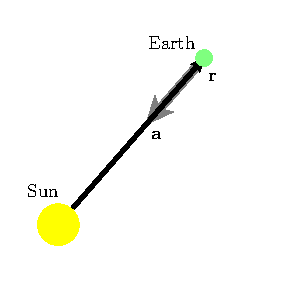
\includegraphics{figures/fig_9_7_sun.eps}
    \caption{A central force.}
    \label{F:9.7.sun}
  \end{center}
\end{figure}

\ba
\item If an object of mass $m$ is moving under a central force, 
  the angular momentum vector is defined to be $\vL=m\vr\times\vv$.
  Assuming the mass is constant, show that the angular momentum is
  constant by showing that
  $$
  \frac{d\vL}{dt} = \vzero.
  $$

\item Explain why $\vL\cdot\vr = 0$.

\item Explain why we may conclude that the object is constrained to
  lie in the plane passing through the origin and perpendicular to
  $\vL$.

\ea

\begin{exerciseSolution}
\ba
\item Since the acceleration is parallel to the position under a central force, if follows that $\vr \times \va = \vzero$. By the product rule we have that 
\begin{align*}
\frac{d\vL}{dt} &= \frac{d}{dt} m\vr\times\vv \\
	&= (m\vr \times \vv') + (m\vr' \times \vv)  \\
	&= m(\vr \times \va) + m(\vv \times \vv) \\
	&= \vzero.
\end{align*}
Since the derivative of $\vL$ is $\vzero$, it follows that $\vL$ is constant. 
  

\item Recall that the cross product of two vectors is perpendicular to both vectors, so $\vL = m(\vr\times\vv)$ is perpendicular to $\vr$. Thus, $\vL\cdot\vr = 0$.

\item Since $\vL = m(\vr \times \vv$ is constant, the position and velocity vectors lie in a single plane perpendicular to $\vL$. To the objects position and motion are constrained to lie in the plane passing through the origin and perpendicular to $\vL$.

\ea
\end{exerciseSolution}


\end{exercises}
\afterexercises


